\documentclass[12pt,a4paper]{report}

% === PACKAGES ===
\usepackage[utf8]{inputenc}
\usepackage[T1]{fontenc}
\usepackage[english]{babel}
\usepackage{graphicx}
\usepackage{hyperref}
\usepackage{geometry}
\usepackage{fancyhdr}
\usepackage{titlesec}
\usepackage{booktabs}
\usepackage{longtable}
\usepackage{array}
\usepackage{xcolor}
\usepackage{listings}
\usepackage{float}
\usepackage{caption}
\usepackage{subcaption}
\usepackage{rotating}
\usepackage{chngcntr}
\usepackage[style=ieee,backend=biber]{biblatex}

% === CONFIGURATION ===
\geometry{margin=2.5cm}

% Remove "Chapter" word from chapter titles
\titleformat{\chapter}[block]{\normalfont\huge\bfseries}{\thechapter.}{1em}{}

% Continuous numbering for figures and tables (1, 2, 3 instead of 4.1, 5.1)
\counterwithout{figure}{chapter}
\counterwithout{table}{chapter}
\hypersetup{
    colorlinks=true,
    linkcolor=blue,
    filecolor=magenta,
    urlcolor=cyan,
    citecolor=blue
}

% Graphics path
\graphicspath{{images/}}

% Bibliography file
\addbibresource{references.bib}

% Header/Footer style
\pagestyle{fancy}
\fancyhf{}
\fancyhead[L]{\leftmark}
\fancyhead[R]{AIutami}
\fancyfoot[C]{\thepage}
% Remove "CHAPTER" from header, show only chapter number and title
\renewcommand{\chaptermark}[1]{\markboth{\thechapter. #1}{}}

% Code listing style
\lstset{
    basicstyle=\ttfamily\small,
    breaklines=true,
    frame=single,
    numbers=left,
    numberstyle=\tiny\color{gray},
    keywordstyle=\color{blue},
    commentstyle=\color{green!60!black},
    stringstyle=\color{orange}
}

% === DOCUMENT INFO ===
\title{\Huge\textbf{AIutami}}
\author{
    Salvatore Pio Conte \\
    Simone Cosenza \\
    Sara Imparato
}
\date{\today}

% === DOCUMENT ===
\begin{document}

% Cover and Abstract
% === COVER PAGE ===
\begin{titlepage}
    \centering
    \vspace*{2cm}

    % Logo placeholder
    % 
\includegraphics[width=0.3\textwidth]{logo.png}

    \vspace{1cm}

    {\Huge\textbf{AIutami}}

    \vspace{0.5cm}

    {\Large AI-Moderated Voice Conference Platform}

    \vspace{2cm}

    {\large
    \begin{tabular}{l l}
        \textbf{Salvatore Pio Conte} & salvatore.conte@example.com \\
        \textbf{Simone Cosenza} & simone.cosenza@example.com \\
        \textbf{Sara Imparato} & sara.imparato@example.com \\
    \end{tabular}
    }

    \vfill

    % === ABSTRACT ===
    \begin{minipage}{0.9\textwidth}
        \textbf{Abstract}\\[0.5em]
        \small
        AIutami is a web-based platform that introduces an AI moderator into vocal group discussions, designed to improve fairness, structure, and conversational flow. The system manages turn-taking to ensure only one participant speaks at a time, monitors conversational dynamics in real time, and intervenes contextually when discussions become unbalanced, stuck, or unfocused. Built on WebRTC for real-time audio streaming, automatic speech recognition for live transcription, and large language models for intelligent moderation, AIutami acts as a neutral facilitator: it listens, understands the flow, and guides the group toward productive outcomes without taking over the conversation. The platform addresses common challenges in group discussions—unequal participation, interruptions, and loss of focus—that current conferencing tools fail to handle in real time. By combining voice interaction with adaptive AI moderation, AIutami brings structure and fairness to collaborative scenarios such as study groups, team meetings, and decision-making activities.
    \end{minipage}

    \vspace{1cm}

    % University/Course info placeholder
    % {\large University Name}\\
    % {\large Course Name}\\
    % {\large Academic Year 2024/2025}

    {\large \today}

\end{titlepage}

\newpage


% Table of Contents
\tableofcontents
\newpage

% The Team
% === THE TEAM ===
\chapter{The Team}

\begin{center}
    \begin{minipage}[b]{0.3\textwidth}
        \centering
        
\includegraphics[height=5cm,keepaspectratio]{team/salvatore.jpg}\\[0.5em]
        \textbf{Salvatore Pio Conte}
    \end{minipage}
    \hfill
    \begin{minipage}[b]{0.3\textwidth}
        \centering
        
\includegraphics[height=5cm,keepaspectratio]{team/simone.jpg}\\[0.5em]
        \textbf{Simone Cosenza}
    \end{minipage}
    \hfill
    \begin{minipage}[b]{0.3\textwidth}
        \centering
        
\includegraphics[height=5cm,keepaspectratio]{team/sara.jpg}\\[0.5em]
        \textbf{Sara Imparato}
    \end{minipage}
\end{center}


% Members' Contribution
% === MEMBERS' CONTRIBUTION ===
\chapter{Members' Contribution}

The following table summarizes each team member's role and responsibilities in the project.

\begin{longtable}{|p{4cm}|p{2cm}|p{8cm}|}
    \hline
    \textbf{Member} & \textbf{Role} & \textbf{Tasks} \\
    \hline
    \endfirsthead

    \hline
    \textbf{Member} & \textbf{Role} & \textbf{Tasks} \\
    \hline
    \endhead

    Salvatore Pio Conte &
    R &
    Backend architecture and implementation (Django, WebSocket, WebRTC, ASR integration), DevOps and deployment (Docker, Azure), contributor to UX design and prompt engineering
    \\
    \hline

    Simone Cosenza &
    R &
    Frontend development (React), UX design (user workflows, scenarios, interaction design), UNG model definition, testing and QA (functional testing, usability), prompt engineering for AI moderation
    \\
    \hline

    Sara Imparato &
    R &
    Frontend development (React), UX design (user workflows, scenarios, interaction design), UNG model definition, testing and QA (functional testing, usability), prompt engineering for AI moderation
    \\
    \hline

\end{longtable}

\textbf{Legend:} R = Responsible (primary owner), C = Contributor (supporting role)


% Executive Summary
% === EXECUTIVE SUMMARY ===
\chapter{Executive Summary}

Group conversations often fail to achieve their potential. Participants interrupt each other, some voices dominate while others remain unheard, and discussions frequently drift off track~\cite{Diehl1987ProductionBlocking}. These dynamics undermine collaboration, making it difficult for groups to share knowledge effectively or reach clear decisions.

AIutami addresses these challenges through an AI-moderated discussion platform. The system allows users to create and join audio-based sessions through a web interface. Each session follows a structured workflow: participants gather in a lobby phase before entering the active discussion. During the conversation, speaking turns are regulated through a request-based mechanism that prevents overlap and ensures balanced participation. Visual feedback keeps participants informed about the current speaker and turn status, improving coordination and reducing confusion.

What distinguishes AIutami from traditional conferencing tools is its intelligent moderation layer. The platform combines real-time audio streaming, automatic speech recognition, and large language models to monitor conversational dynamics. When the discussion becomes unbalanced, stuck, or loses focus, the AI moderator intervenes contextually---prompting quieter participants, redirecting off-topic exchanges, or helping the group move forward.

Consider a Murder Mystery activity where participants must share clues and collaborate to identify the culprit. Without structure, a few voices dominate, clues get lost, and the group struggles to reason together. With AIutami, every participant gets heard, key points remain visible, and the group can build toward a shared conclusion. The same benefits apply to study groups debating complex topics, teams making strategic decisions, or workshops requiring structured input from all participants.

AIutami delivers concrete value: discussions that are fairer, more focused, and more likely to produce clear outcomes.


% Requirements
% === REQUIREMENTS ===
\chapter{Requirements}

This chapter describes the project requirements following the UNG model, which structures the analysis around Users (stakeholders), their Needs, and the system Goals that address those needs, all within a specific Context and subject to Constraints. The accompanying UNG diagram visualizes the relationships between these elements.

\section{Target Groups and Stakeholders}

The system addresses three levels of stakeholders based on their proximity to the platform and their role in the interaction.

\textbf{Primary users} are the direct participants in moderated discussions. This group includes students and researchers engaging in academic debates or group projects, colleagues collaborating in professional meetings, and participants in educational or entertainment activities.

\textbf{Secondary users} are those who oversee discussions without being the main speakers. This category includes teachers and trainers who monitor student participation, team leaders and managers who guide collaborative sessions, and facilitators who use the system as a support tool for group dynamics.

\textbf{Tertiary users} are individuals or organizations that do not interact directly with the platform but are affected by its adoption. These include educational institutions and companies that deploy the system to improve internal collaboration.

\textbf{MVP Focus:} For the purpose of this project, the implementation targets the Murder Mystery experimental paradigm~\cite{Stasser1992HiddenProfiles}, where participants must collaborate vocally to solve a case. This context was chosen because it naturally exhibits the challenges the system aims to address: multiple voices competing to speak, risk of dominant participants, and the need for structured turn-taking to reach a shared conclusion.

\section{Stakeholder Needs}

The needs addressed by AIutami emerge from the typical dynamics of group vocal conversations, where communication imbalances, interruptions, and lack of inclusion often occur.

\textbf{Feeling heard and included} --- Participants need equitable speaking opportunities without some voices monopolizing the conversation.

\textbf{Communicating clearly and fluidly} --- Groups need to reduce interruptions, overlaps, and confusion that disrupt the natural flow of discussion.

\textbf{Maintaining focus and productivity} --- Discussions often drift off-topic; participants need support to stay on track and reach shared conclusions.

\textbf{Participating with confidence} --- Some participants feel hesitant to speak, especially in groups with dominant personalities. They need an environment that encourages balanced contribution.

\textbf{Observing and improving group communication} --- Secondary users such as facilitators and teachers need tools to monitor participation patterns and guide the conversation effectively.

\textbf{Ensuring transparency} --- Users need to understand when the AI is listening and how their contributions are being processed.

\section{Context}

The context describes where and how the system is used, articulated across four dimensions.

\textbf{Organizational context} --- AIutami supports structured collaborative phases such as group study sessions, team meetings, brainstorming activities, and educational workshops. The system acts as a vocal facilitator during these interactions.

\textbf{Physical context} --- The platform is a web-based application accessible through standard browsers. Users need a microphone or headset for audio input, a stable internet connection (approximately 10 Mbps), and low network latency (under 200ms) to ensure real-time responsiveness.

\textbf{Temporal context} --- The system operates primarily in real-time mode, monitoring and intervening vocally during active discussions. At the end of each session, a summary report is generated to capture key outcomes.

\textbf{Social context} --- AIutami is designed for small groups of 2 to 8 participants. These groups may have equal roles (peers collaborating) or differentiated roles (teacher-students, team leader-colleagues). The shared objective is typically collaborative decision-making, learning, or structured discussion.

\textbf{MVP Scope:} The current implementation focuses on the Murder Mystery experimental scenario with 3 participants collaborating to solve a case through structured vocal interaction.

\section{Goals}

The goals represent the functional objectives that the system must achieve to address user needs. While needs describe what users require, goals describe what the system does to satisfy those requirements.

\textbf{Manage turn-taking fluidly} --- The system regulates speaking turns through a request-based mechanism, ensuring only one participant speaks at a time and preventing overlaps. Visual feedback indicates the current speaker and turn status.

\textbf{Identify participants through the turn system} --- Rather than using voice recognition to identify speakers, the system tracks who is speaking based on who holds the current turn. This approach associates each transcribed contribution with the correct participant.

\textbf{Provide real-time vocal feedback} --- The AI moderator intervenes with synthesized voice messages when discussions become unbalanced, stuck, or unfocused. These interventions prompt quieter participants, redirect off-topic exchanges, or help the group move forward.

\textbf{Summarize key points} --- The system generates vocal summaries during and at the end of sessions, highlighting main discussion points and outcomes. A final report preserves these summaries for future reference.

\textbf{Monitor participation levels} --- The system tracks speaking time and turn distribution across participants, enabling balanced contribution and providing data for secondary users to assess group dynamics.

\section{Constraints}

Several factors constrain the system's design and performance.

\textbf{Potential latency in the processing chain} --- The system relies on a sequential pipeline: speech recognition (ASR), language model processing (LLM), and voice synthesis (TTS). Each step introduces potential delays, particularly if the LLM response is slow. While current performance is acceptable, network conditions or service load could affect real-time responsiveness.

\textbf{Speech recognition accuracy} --- The ASR service may produce transcription errors, particularly with background noise, accents, or unclear speech. While occasional errors are acceptable, they can affect the quality of summaries and the AI's understanding of the discussion.

\textbf{LLM behavioral limitations} --- The language model powering the AI moderator has limited customization. Content moderation policies and inherent model behaviors may occasionally produce responses that are not perfectly suited to the moderation context.

\textbf{Cloud-based audio processing} --- Audio data is transmitted to external cloud services (Azure Speech) for transcription. While these services follow industry security standards, users should be aware that their voice data is processed externally. The system does not store raw audio or full transcriptions---only session summaries are retained for the final report.

\section{UNG Diagram}

\begin{figure}[H]
    \centering
    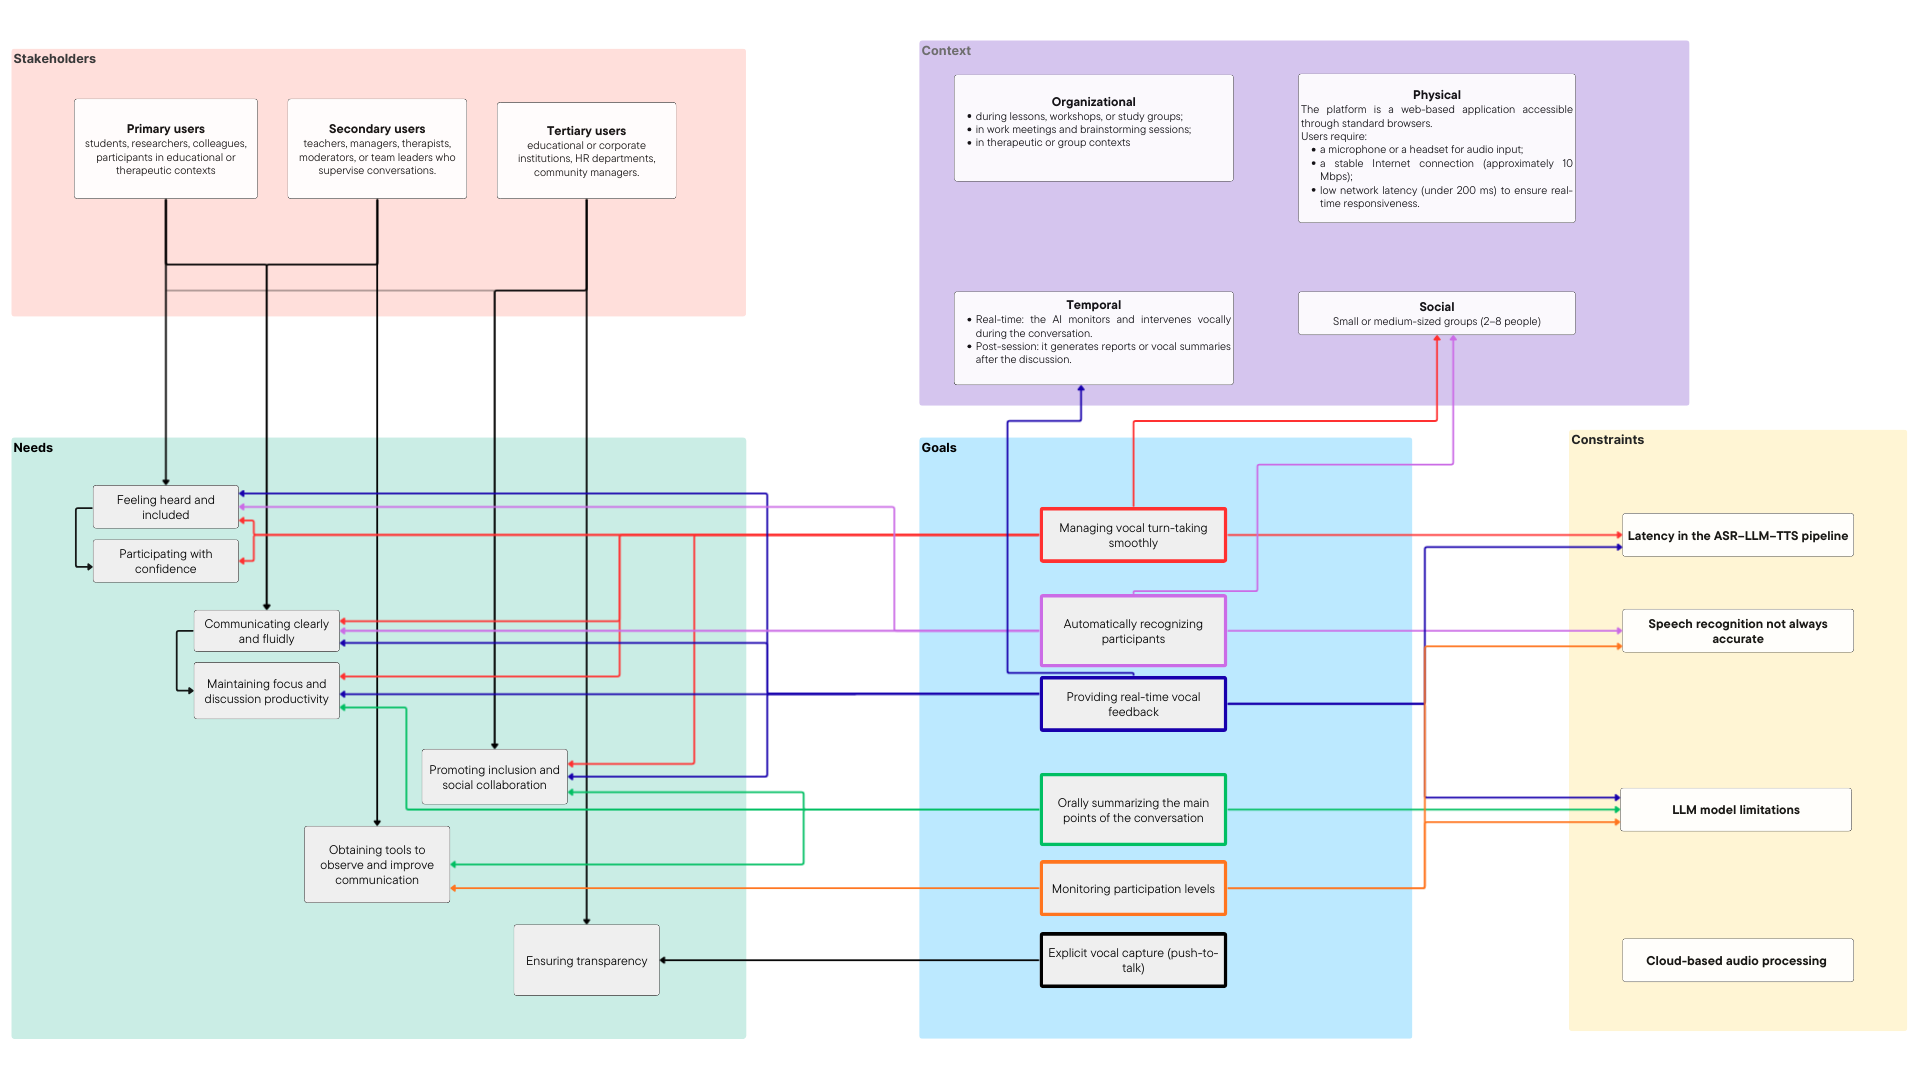
\includegraphics[angle=90,width=\textwidth,height=0.85\textheight,keepaspectratio]{ung-diagram.png}
    \caption{UNG Diagram showing the relationships between stakeholders, needs, goals, context, and constraints.}
    \label{fig:ung}
\end{figure}


% State of the Art
% === STATE OF THE ART ===
\chapter{State of the Art}

This chapter analyzes related academic works, existing commercial products, and identifies open research directions relevant to the AIutami project.

\section{Related Works}

\textbf{LLMs in Multi-User Contexts} --- Research on LLM-based conversational systems has historically focused on dyadic interactions. The Multi-User Chat Assistant (MUCA) framework from Microsoft Research represents one of the first systematic attempts to address multi-user contexts~\cite{Mao2024MUCA}. MUCA introduces the 3W model that formalizes three fundamental dimensions for group chatbots: What (response content), When (timing or strategic silence), and Who (addressing an individual, subgroup, or entire group). The framework identifies recurring challenges in group conversations: stuck discussions, multi-thread management, reactivity control, participation equity, and conflict resolution. Its modular architecture combines topic generation, dialog analysis, and strategy arbitration. Results show improvements in intervention timing and perceived quality compared to single-prompt approaches, though the framework operates exclusively in the text domain.

\textbf{AI-Based Moderation and Facilitation} --- Group discussion moderation has traditionally relied on human facilitators or rigid rule-based systems. The thesis ``Multiuser Conversational Agents Based on Large Language Models''~\cite{Dubini2024MultiuserConversationalAgents} represents pioneering work exploring LLM-based moderation. The study analyzes a GPT-3.5 moderator using the Hidden Profile experimental paradigm---a collaborative decision-making task where participants possess partial, unique information, requiring effective discussion to reach the correct solution. Results show that the AI moderator influences conversation structure and participation patterns, though it does not significantly improve decision accuracy. The work identifies key limitations: task-agnostic moderators may suggest unrealistic actions, participant motivation affects outcomes, and standard evaluation metrics are lacking. The thesis concludes that LLM moderation is promising but requires greater task contextualization. A subsequent study, ``Large Language Models as Facilitators in Multi-user Conversations''~\cite{Anonymous2026LLMFacilitators}, extends these findings using a GPT-4o facilitator with minimal prompt engineering. Participants with the facilitator achieve higher individual accuracy. The analysis identifies emergent functions: conversational regulation, task-specific guidance, bias reduction, and time management. However, occasional hallucinations and premature time pressure remain problematic.

\textbf{LLM Limitations in Multi-Turn Conversations} --- The paper ``LLMs Get Lost in Multi-Turn Conversation''~\cite{Laban2025LLMsGetLost} addresses a critical limitation relevant to moderation systems. The study demonstrates that LLM performance degrades as conversational turns increase, even without semantic ambiguity. This loss of conversational state tracking manifests through forgotten constraints, contradictions with past statements, and locally correct but globally incoherent responses. Neither larger context windows nor bigger models resolve the issue. The authors attribute this to structural factors: LLMs lack explicit dialogue state representation and treat context as unstructured text. The implication is clear: robust conversational systems require structured memory and explicit state tracking beyond pure prompting approaches.

\section{Existing Products}

Commercial video conferencing platforms such as Zoom, Microsoft Teams, and Google Meet provide real-time audio communication but lack intelligent moderation. Turn-taking is manual, participation balance is not monitored, and no AI-driven facilitation exists.

Transcription services like Otter.ai focus on documentation rather than active intervention. Conversation intelligence platforms such as Gong operate retrospectively on recorded calls rather than in real-time.

No commercial product currently combines real-time voice conferencing with AI-based moderation for group discussions.

\section{Gap Analysis}

The literature review reveals open directions in LLM-based conversational systems.

\textbf{Modality} --- Existing research focuses on text-based conversations, while commercial products handle voice without intelligent moderation. The intersection---real-time voice moderation---remains largely unexplored.

\textbf{Context Awareness} --- Research indicates that task-agnostic moderators produce suboptimal interventions. Approaches balancing LLM flexibility with domain awareness represent an open area.

\textbf{Architectural Robustness} --- Studies show that prompt-only systems struggle with state coherence in extended conversations. Integrating structured memory with conversational AI is an active research direction.

AIutami positions itself within these open spaces, exploring an architecture that combines voice-based interaction, contextual moderation, and explicit state management.


% Solution - UX Design
% === SOLUTION - UX DESIGN ===
\chapter{Solution - UX Design}

\section{General Approach}

The UX design of AIutami follows a core principle: minimize interface complexity so that participants can focus entirely on the conversation. As a real-time voice platform, every interface element is designed to be immediately understandable without prior instruction.

The interaction follows a sequential phase model---registration, session creation or joining, lobby, active discussion, conclusion, and session closure---each with a dedicated interface that displays only the actions available at that stage. This approach reduces cognitive load: users never face unnecessary choices or ambiguous options.

During the active discussion phase, the interface centers on a single primary element: the push-to-talk button. The choice of push-to-talk over an always-open microphone is deliberate: it makes the act of ``taking the floor'' an explicit gesture, aligning the digital interaction with the natural dynamics of a moderated conversation. Visual indicators display who is currently speaking, who has reserved the next turn, and the AI moderator's status.

The AI moderator is integrated into the experience as an additional participant rather than a separate control panel. It intervenes vocally when needed---prompting quieter users, redirecting off-topic exchanges, or signaling phase transitions---without requiring users to interact with it through commands or text input. Moderation happens transparently, driven by real-time analysis of the conversation's transcription and participation patterns.

\section{User Workflows}

This section describes the two main workflows that define the user experience in AIutami. The first covers the steps from account creation to the start of a moderated discussion; the second describes the interaction dynamics during and after the discussion.

\subsection{Pre-Session Flow}

\begin{figure}[H]
    \centering
    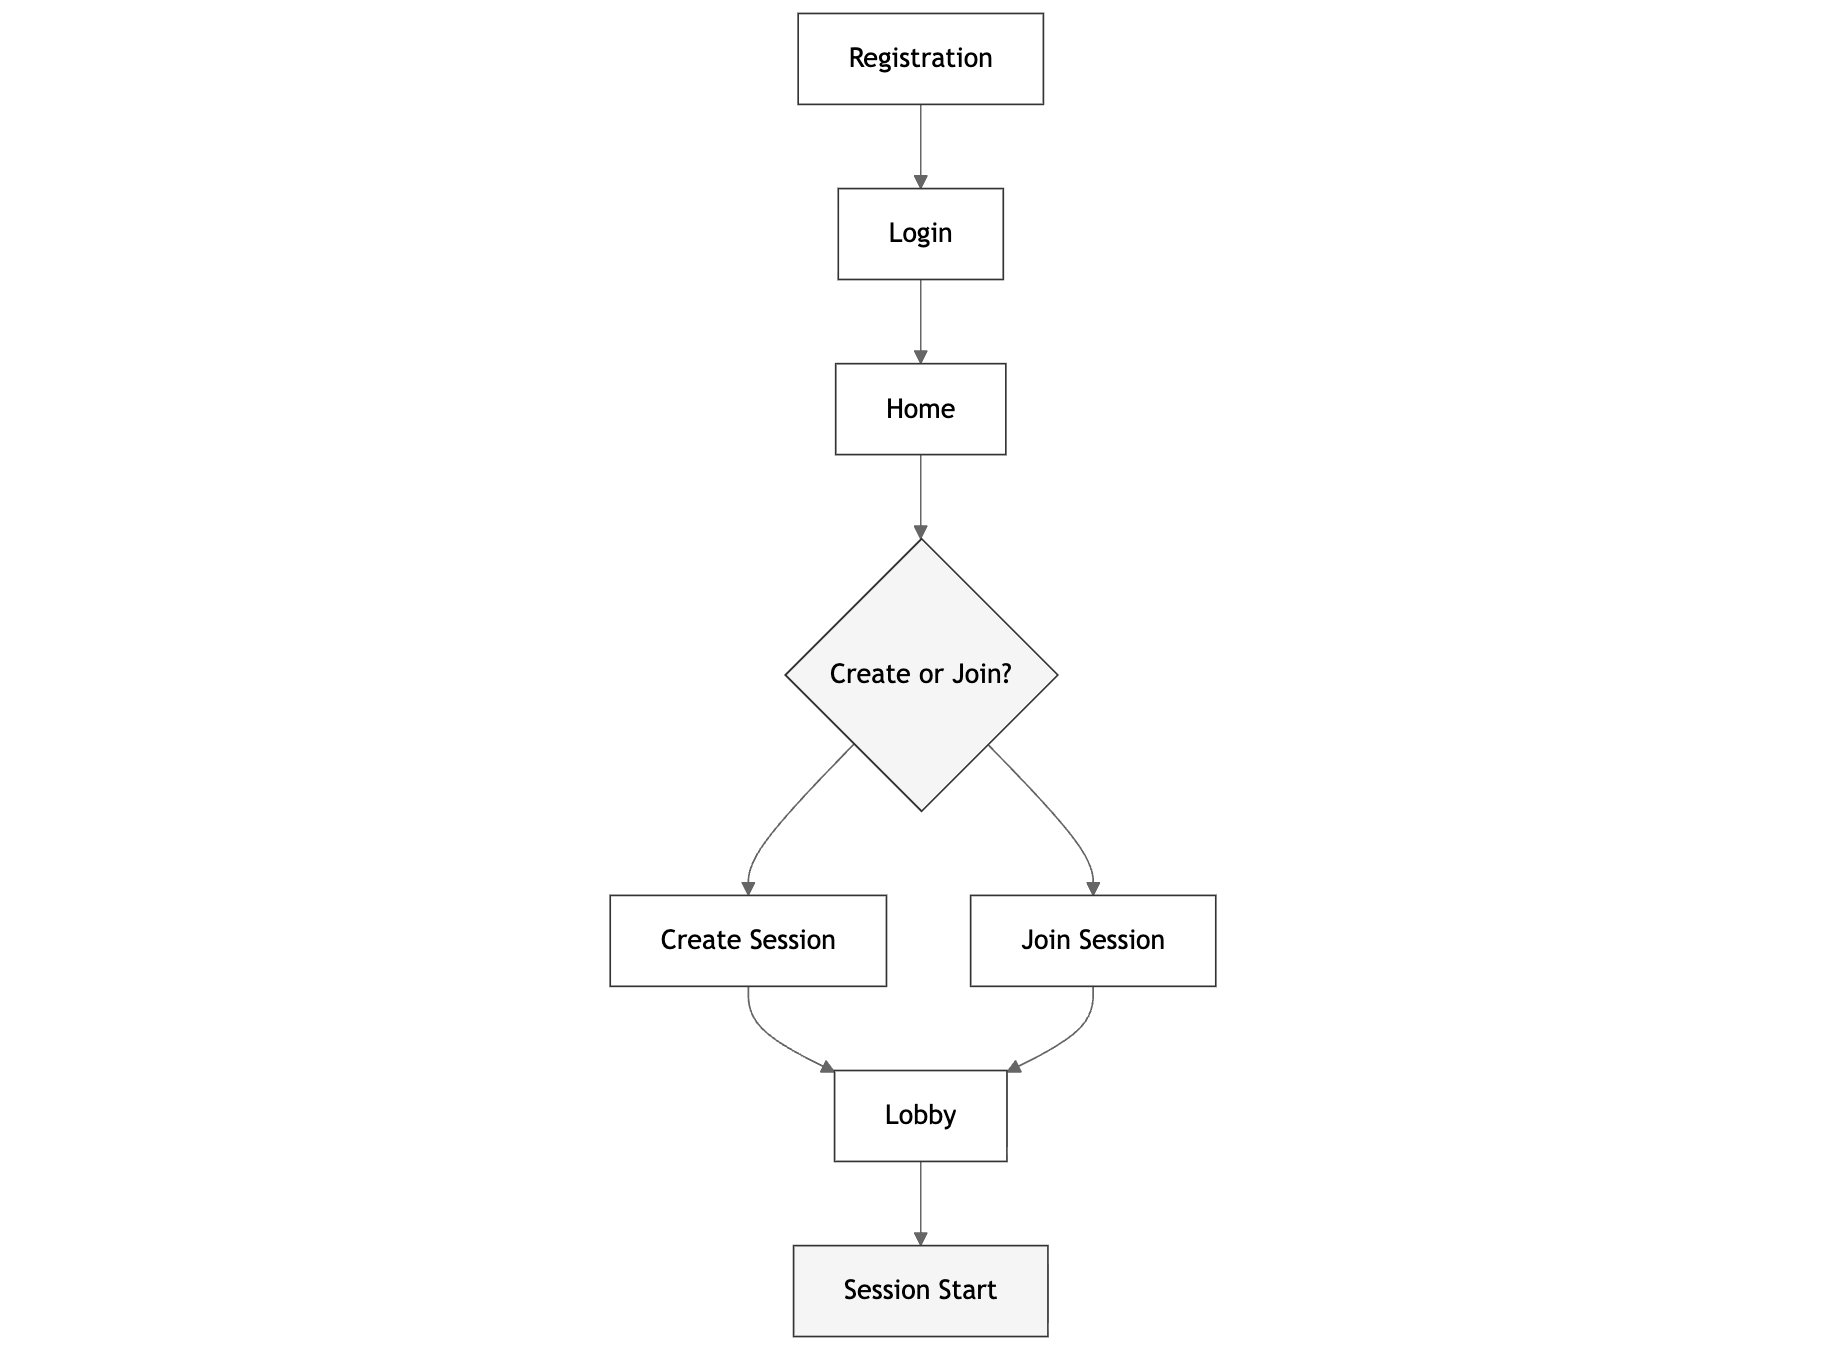
\includegraphics[width=0.9\textwidth]{workflow-pre-session.png}
    \caption{Pre-Session Workflow}
    \label{fig:workflow-pre}
\end{figure}

The pre-session workflow covers all steps from account creation to the start of a moderated discussion.

\begin{enumerate}
    \item \textbf{Registration} --- The user creates an account by providing name, surname, email, username, and password. The account is immediately active upon successful registration.
    \item \textbf{Login} --- The user authenticates with email and password, obtaining access to the platform.
    \item \textbf{Home} --- The user accesses the main view, which presents three options: create a new session, join an existing session via invitation link, or browse past sessions.
    \item \textbf{Create Session} (path A) --- The user selects a discussion context (Murder Mystery, Academic, Therapeutic, or Workplace), enters a session title, and confirms. The system creates the session and redirects the user to the lobby as host.
    \item \textbf{Join Session} (path B) --- The user pastes an invitation link received from a host. The system validates the link and adds the user to the session's lobby.
    \item \textbf{Lobby} --- All participants wait in the lobby. The host can see the participant count and, once the required number of participants has joined, starts the session.
    \item \textbf{Session Start} --- The AI moderator delivers an introductory message explaining the rules and the discussion begins.
\end{enumerate}

\subsection{In-Session Flow}

\begin{figure}[H]
    \centering
    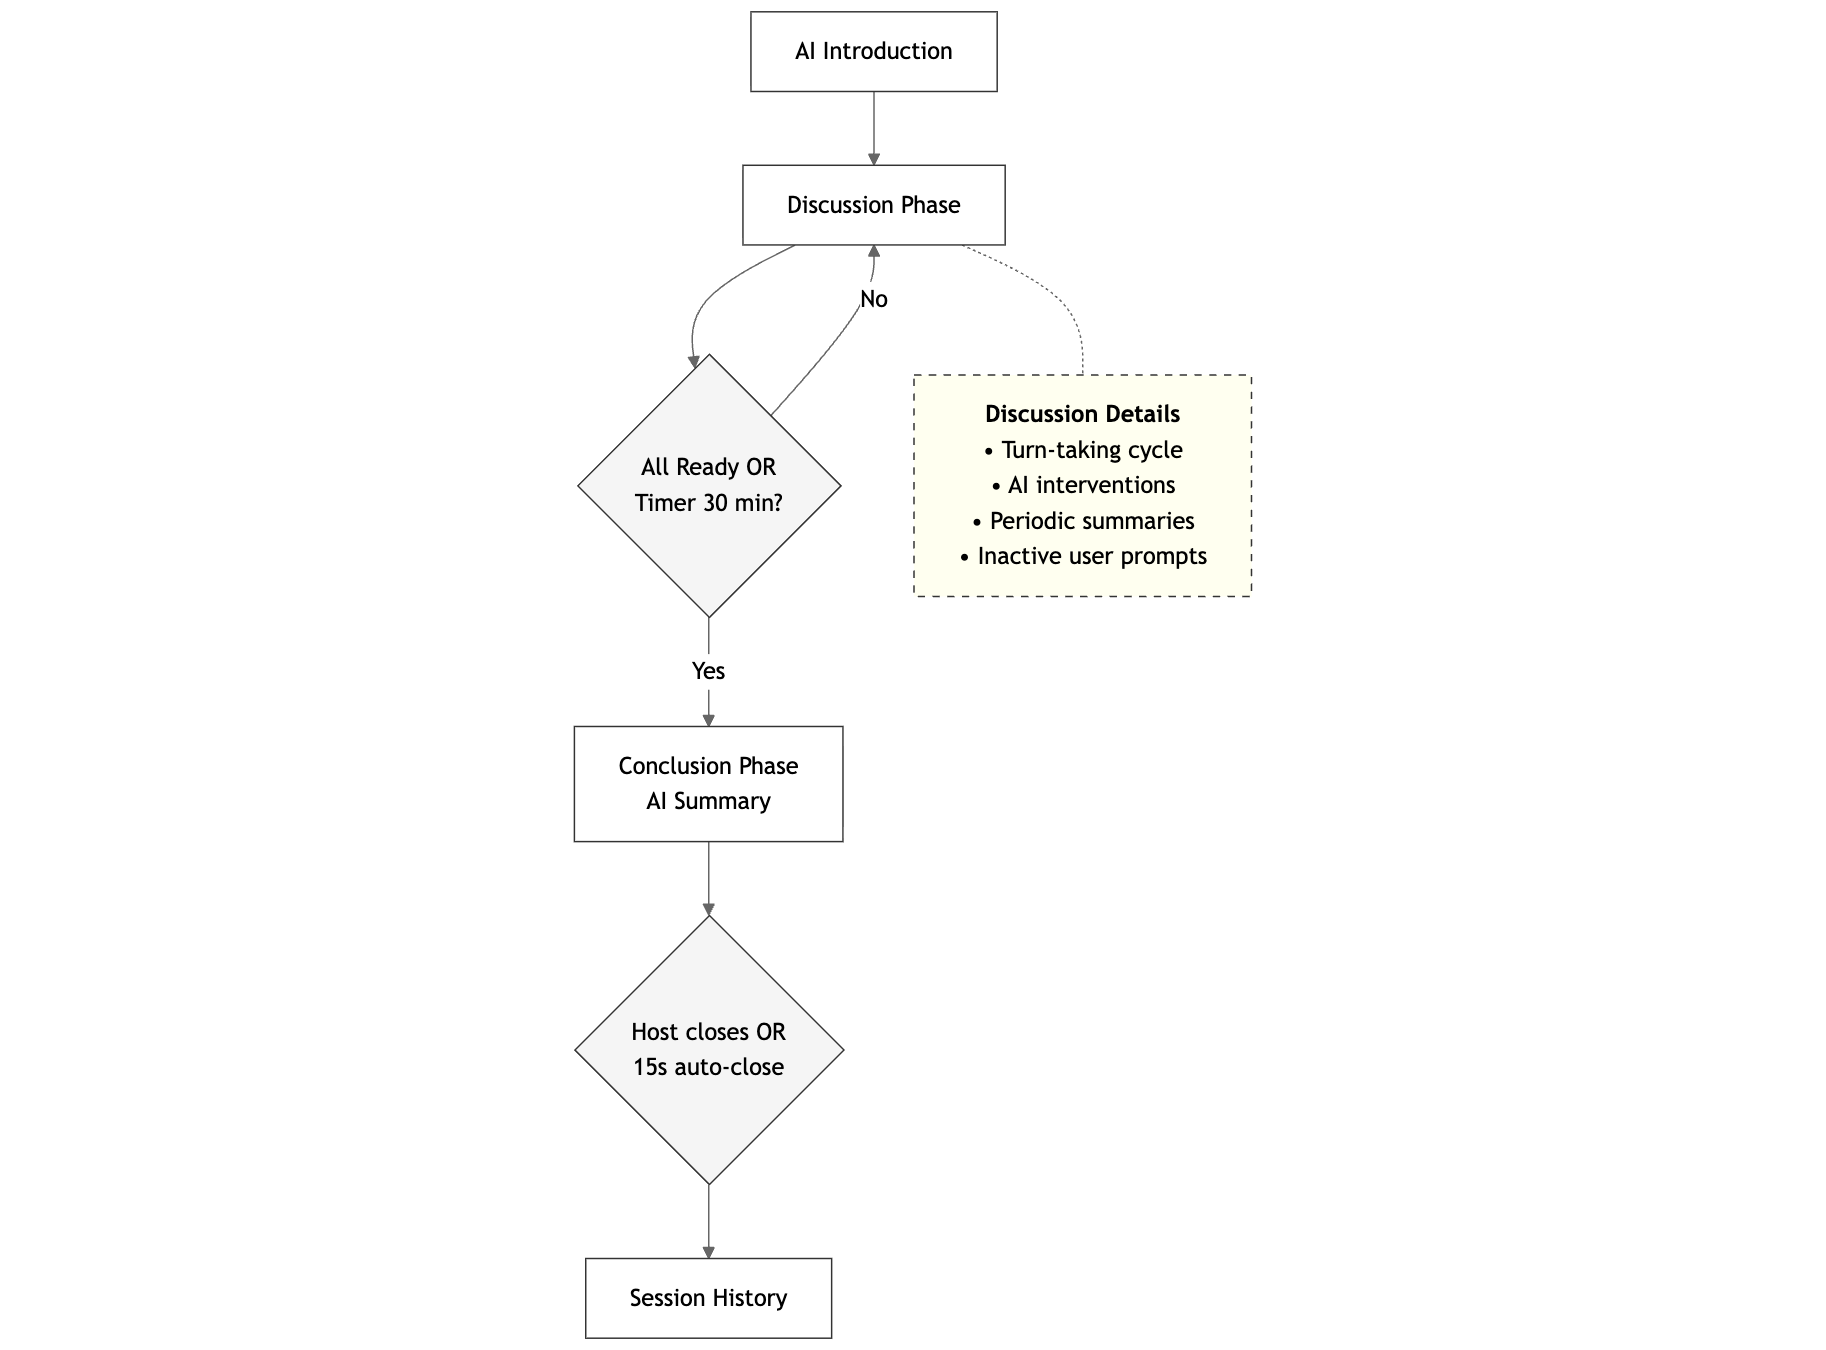
\includegraphics[width=0.9\textwidth]{workflow-in-session.png}
    \caption{In-Session Workflow}
    \label{fig:workflow-in}
\end{figure}

The in-session workflow describes the interaction dynamics from the start of the discussion to session closure.

\begin{enumerate}
    \item \textbf{AI Introduction} --- The moderator welcomes participants, explains the interaction rules, and opens the discussion.
    \item \textbf{Discussion Phase} --- Participants engage in conversation through a turn-taking system: one speaks via push-to-talk while others can reserve the next turn with an 8-second priority window. Throughout the discussion, the AI moderator monitors participation and intervenes when needed---delivering periodic summaries, prompting inactive users, or addressing collective silence.
    \item \textbf{Conclusion Phase} --- Triggered when all participants declare readiness or when the 30-minute timer expires. The moderator delivers a vocal summary of the discussion. In the Murder Mystery context, this is followed by a voting phase where participants select the suspect they believe is guilty.
    \item \textbf{Session Closure} --- The host closes the session manually, or the system closes it automatically after 15 seconds. A final report is generated.
    \item \textbf{Session History} --- The session appears in each participant's history, where the report can be viewed and downloaded as PDF.
\end{enumerate}

\section{User Scenarios}

This section presents a series of user scenarios that illustrate the main interactions with the platform, from registration to session closure.

\subsection{Scenario 1: A New User Registers}

Luca, a new user interested in participating in moderated discussions on AIutami, decides to sign up. He accesses the homepage and selects the ``Sign up'' option.

He fills in the registration form with his first name, last name, email address, username, and password. After submitting the form, AIutami verifies that the chosen username and email address are not already associated with an existing account. Upon successful validation, Luca's account is immediately created and active.

Luca is redirected to the login page, where he enters his credentials to access the platform for the first time. Once authenticated, he reaches the home page, from which he can create a new voice session, join a session via an invitation link, or browse the history of completed sessions.

\subsection{Scenario 2: A Registered User Logs In}

Marco, an existing user of AIutami, wants to access his account. From the homepage he selects ``Log in'' and enters his email and password. The system verifies his credentials and, once authenticated, redirects him to the home page. From here he can view active sessions, create a new one, join an existing session through an invitation link shared by another participant, or browse the history of past sessions.

\subsection{Scenario 3: Creating a New Session}

Luca, who has just logged in to AIutami, wants to start a new session to discuss with other users. From the home page, he selects ``Create new session'' and is redirected to the session configuration page.

Here he chooses one of the available discussion contexts---Murder Mystery, Academic, Therapeutic, or Workplace---and enters a title for the session. Once confirmed, the system creates the session and redirects Luca to the lobby as host.

From the lobby, Luca generates an invitation link and shares it with the other participants he wants to invite. The lobby displays in real time the list of participants who have joined. Luca waits until the required number of participants has connected before starting the discussion.

\subsection{Scenario 4: Joining a Session}

Giovanni, who is already logged in to AIutami, wants to join a session created by his friend Luca. From the home page, he selects ``Join with a link'' and is redirected to the join page, where he finds a text field to paste the invitation link received from Luca. After pasting it, he confirms by clicking ``Join session.''

The system validates the link and checks that the session is still in the lobby phase and has not reached its maximum number of participants. If successful, Giovanni is redirected to the lobby, where he can see the list of participants already connected and wait for the host to start the discussion.

\subsection{Scenario 5: Starting a Session}

Marco, the host of a Murder Mystery session on AIutami, is in the lobby together with the invited participants, Luca and Giovanni. In this context, the number of participants is fixed at three, so the interface displays a counter indicating how many users have joined.

When the counter reaches the required number, Marco selects the ``Start session'' button, visible only to him as host. The session enters its active phase and all participants are redirected to the discussion interface.

The AI moderator takes the floor to introduce the session: it welcomes the participants, explains the interaction rules, and opens the discussion.

\subsection{Scenario 6: Speaking During a Session}

Marco, a participant in an active session on AIutami, wants to open the conversation. He presses the push-to-talk button to activate his microphone. The interface visually indicates that his turn is active, while the other participants can only reserve their turn to speak next.

Marco shares his thoughts and, once finished, selects the ``End turn'' button, releasing the floor. From that moment, any participant can press the push-to-talk button to take the next turn.

\subsection{Scenario 7: Reserving the Next Turn}

Giovanni, a participant in the same session, wants to speak while Marco is talking. From his interface, he presses the ``Reserve turn'' button, which is available only when another participant holds the floor.

The system registers his request. When Marco ends his turn, Giovanni receives an 8-second priority window during which only his push-to-talk button is active. Giovanni presses it within this interval and begins speaking. After he finishes and ends his turn, the floor becomes available to all participants again.

\subsection{Scenario 8: Inactive User}

Giovanni is in a session together with Luca and Marco. The discussion is about a project update and proceeds at a steady pace: Luca and Marco alternate speaking turns while Giovanni listens in silence without ever pressing the push-to-talk button.

After several minutes of inactivity, a private text notification appears on Giovanni's screen, inviting him to participate in the conversation. Giovanni reads the message but chooses not to speak and lets the others continue.

After further minutes of inactivity, the AI moderator intervenes vocally, addressing Giovanni by name and encouraging him to share his thoughts with the group. Giovanni decides to accept the invitation, presses the push-to-talk button, and contributes his perspective to the discussion.

\subsection{Scenario 9: Ready to Conclude (Murder Mystery)}

Chiara, a participant in a Murder Mystery session, has been collaborating with Matteo and Silvia to identify the culprit. After several exchanges, Chiara believes she has found a possible solution and presses the ``Ready to conclude'' button.

The system registers her action and the AI moderator announces to the group that Chiara is ready to propose a conclusion. Chiara continues participating in the discussion while Matteo and Silvia keep deliberating.

Eventually, Matteo also presses the button, and the moderator announces his declaration. When Silvia, the last remaining participant, presses ``Ready to conclude'' as well, the moderator announces that all participants are ready and the session transitions to the conclusion phase. The AI moderator delivers a vocal summary of the discussion, recapping the main points and clues that emerged.

\subsection{Scenario 10: Voting (Murder Mystery)}

After the AI moderator has delivered the discussion summary, the session enters the voting phase. Each participant sees a voting interface presenting the list of suspects. Chiara, Matteo, and Silvia must each select the character they believe is the culprit.

Chiara casts her vote first. The system registers her choice and notifies the group that she has voted, without revealing her selection. Matteo and Silvia follow. Once all three participants have voted, the system reveals the results: each participant's choice, the correct answer, and whether the group successfully identified the culprit.

\subsection{Scenario 11: Time Running Out}

During an active session on AIutami, Giulia is participating in a Workplace discussion. The maximum session duration is 30 minutes, visible in the interface.

When the elapsed time reaches 25 minutes, a text notification appears on each participant's screen, informing them that approximately five minutes remain before the conclusion phase begins. Giulia reads the message and dismisses it, returning to the discussion.

When the 30-minute mark is reached, the AI moderator intervenes vocally to announce that the discussion time has ended. The session transitions to the conclusion phase: the moderator delivers a vocal summary of the key points and outcomes of the conversation, and the session proceeds to its closing steps.

\subsection{Scenario 12: Session Closure and Report}

After all participants have cast their votes in the Murder Mystery session, Marco, as host, selects the ``Close session'' button. The system generates a final report containing the session details, voting results, and an analysis of the discussion. Marco is redirected to the session history.

Later, Sara, one of the participants, wants to share the session outcome with her professor. From the home page, she selects ``Session history'' and locates the completed session. On the detail page she can view the session creator, participants, duration, voting results, and the summary generated by the AI moderator. She downloads the report as PDF and sends it to her professor.

\section{Conversational Interaction}

The AI moderator in AIutami acts as a neutral vocal facilitator that participates in the discussion alongside human users. It does not express opinions on the topic being discussed, nor does it take sides. Its role is exclusively procedural: ensuring balanced participation, maintaining focus, and guiding the group through the session's phases.

The moderator communicates through synthesized voice messages delivered via the same audio channel used by human participants. This design choice makes the moderator's presence natural within the conversation flow, rather than relying on text overlays or separate notification systems. When the moderator speaks, the interface reflects this through the same visual indicators used for human speakers. All interventions follow a principle of minimal intrusiveness: the moderator speaks only when necessary, uses brief and indirect language, and never interrupts a participant who is speaking.

From the user's perspective, the moderator's interventions fall into distinct categories. \textbf{Session-level announcements} occur at key phase transitions: the moderator introduces the session at the start, warns participants when discussion time is running low, and delivers a closing summary when the session moves to its conclusion phase. \textbf{Periodic summaries} provide a brief vocal recap of the main points at regular intervals, optionally including a gentle redirection if the conversation has drifted or participation has become unbalanced. \textbf{Individual engagement} addresses prolonged silence from a specific participant: first through a private text notification visible only to that user, then, if the silence continues, through a vocal prompt addressing them by name. \textbf{Collective silence} handling activates when no participant takes the floor for a prolonged period, encouraging someone to restart the discussion. Finally, \textbf{contextual interventions} are triggered after speaking turns when significant issues are detected---such as monopolization, aggressive tones, or a direct request for help. Minor deviations and civil disagreements do not trigger an intervention.


% Solution - Implementation
% === SOLUTION - IMPLEMENTATION ===
\chapter{Solution - Implementation}

\section{Hardware Architecture}
% TODO: If applicable, describe HW components

\section{Software Architecture}

\subsection{Functional Architecture}
% TODO: High-level functional components
% \begin{figure}[H]
%     \centering
%     \includegraphics[width=0.9\textwidth]{architecture-functional.png}
%     \caption{Functional Architecture}
%     \label{fig:arch-func}
% \end{figure}

\subsection{Implementation Architecture}
% TODO: Technical implementation details
% - Technology stack
% - System components
% - Data flow

% \begin{figure}[H]
%     \centering
%     \includegraphics[width=0.9\textwidth]{architecture-implementation.png}
%     \caption{Implementation Architecture}
%     \label{fig:arch-impl}
% \end{figure}

\subsection{Technology Stack}
% TODO: List and describe technologies used

\begin{itemize}
    \item \textbf{Backend:} Django, Daphne (ASGI)
    \item \textbf{Database:} PostgreSQL
    \item \textbf{Cache/Queue:} Redis
    \item \textbf{Real-time:} WebSocket, WebRTC
    \item \textbf{AI Services:} Azure Speech-to-Text, Azure OpenAI
\end{itemize}

\subsection{Data Flow}
% TODO: Describe how data flows through the system


% Empirical Evaluation
% === EMPIRICAL EVALUATION ===
\chapter{Empirical Evaluation}

% TODO: If evaluation was performed, describe:

\section{Evaluation Goals}
% What did you want to measure?

\section{Variables}
% Which variables were measured?

\section{Participants}
% Profile and number of users involved

\section{Tasks}
% What tasks did participants perform?

\section{Data Gathering Method}
% How was data collected? (surveys, interviews, logs, etc.)

\section{Results}
% Main findings and analysis

% If no evaluation was performed:
% \textit{Empirical evaluation was not performed for this project.}


% Value Proposition
% === VALUE PROPOSITION ===
\chapter{Value Proposition}

\section{Value for Users}

AIutami provides value by addressing a fundamental problem in group discussions: unequal participation. In typical conversations, a few vocal individuals tend to dominate while others remain silent---not because they lack ideas, but because they struggle to find space to speak. This imbalance leads to missed insights, disengaged participants, and decisions that reflect only a subset of the group's collective knowledge.

AIutami solves this through structured turn-taking managed by an AI moderator. The system monitors who has spoken and for how long, gently prompting quieter members to contribute while preventing any single participant from monopolizing the conversation. Periodic summaries keep everyone aligned on what has been discussed, and participation tracking makes imbalances transparent to the group.

The result is a more democratic conversation where all voices are heard. Users no longer need to compete for attention or worry about being interrupted. The AI handles the social friction of turn-taking, freeing participants to focus on the content of the discussion rather than the mechanics of who speaks next.


\section{Why It's a Good Solution}

AIutami's design choices directly address the limitations identified in current research and existing products.

\textbf{Voice-first approach.} While most LLM-based moderation research focuses on text chat, real group discussions happen through voice. AIutami bridges this gap by integrating speech-to-text transcription with AI moderation, enabling intelligent facilitation in the natural medium of spoken conversation.

\textbf{Proactive intervention.} Unlike transcription tools that passively record, AIutami's moderator actively participates. It can prompt quiet members, redirect off-topic discussions, and summarize progress---intervening when helpful rather than merely observing.

\textbf{Structured state management.} Research shows that LLMs struggle with long, multi-turn conversations, losing track of context and constraints over time. AIutami addresses this through explicit turn tracking and conversation state stored in Redis, ensuring the moderator maintains coherent awareness of who has spoken, what has been discussed, and where the conversation stands.

\textbf{Task-aware moderation.} Studies indicate that generic, task-agnostic moderators produce suboptimal interventions. AIutami allows session-specific context and goals, enabling the AI to provide relevant guidance rather than generic facilitation.

\textbf{Balanced automation.} The system automates the mechanics of turn-taking without replacing human agency. Participants remain in control of the content; the AI only manages the structure. This balance preserves natural discussion dynamics while eliminating the friction of manual coordination.

These choices result in a system that is technically grounded in current research while addressing practical gaps in existing tools.


\section{Competitive Landscape}

Existing solutions address fragments of the group discussion problem, but none combines real-time voice with active AI moderation.

Video conferencing platforms like Zoom and Microsoft Teams provide the communication infrastructure and have recently integrated AI assistants for meeting summaries and Q\&A. However, turn-taking remains entirely manual---participants must self-regulate who speaks and when, often resulting in interruptions and unbalanced participation.

Transcription services such as Otter.ai offer real-time speech-to-text and live summaries, but operate as passive observers. They document what is said without influencing how the conversation unfolds.

Conversation intelligence platforms like Gong provide sophisticated analytics and even real-time coaching, but target sales contexts rather than collaborative group discussions.

AIutami occupies a distinct position: it is the only platform designed specifically for structured group discussions with an AI moderator that actively manages turn-taking, monitors participation balance, and intervenes when the conversation needs guidance. Rather than analyzing discussions after they end or documenting them passively, AIutami shapes conversational dynamics as they happen---helping groups reach clear, shared outcomes.


% Discussion and Future Work
% === DISCUSSION AND FUTURE WORK ===
\chapter{Discussion and Future Work}

\section{Critical Reflection}
% TODO: Reflect on the project
% - What worked well?
% - What could be improved?
% - Lessons learned

\section{Limitations}
% TODO: Known limitations of the current implementation

\section{Future Developments}
% TODO: Potential future enhancements
% - Short-term improvements
% - Long-term vision

% Optional: Business Perspectives
% \section{Business Perspectives}
% TODO: If applicable
% - Market opportunity
% - Business model
% - Monetization strategy


% Bibliography
% === BIBLIOGRAPHY ===
\chapter*{Bibliography}
\addcontentsline{toc}{chapter}{Bibliography}

% Print bibliography from references.bib
% Uses IEEE format as required
\printbibliography[heading=none]


% Annexes
% === ANNEXES ===
\appendix
\chapter{Annexes}

% TODO: Add any additional material
% Examples:
% - Screenshots for user manual
% - Detailed prompts for conversational agents
% - Implementation details
% - API documentation

\section{Prompt Examples}
% TODO: If applicable, include detailed prompts used for AI moderation

\section{Screenshots}
% TODO: Additional screenshots

\section{Implementation Details}
% TODO: Technical details not covered in main text


\end{document}
